\section{函数极限的运算}
在下面的讨论中,记号“\(\lim\)”下面没有标明自变量的变化过程,
实际上,下面的定理对\(x \to x_0\)及\(x \to \infty\)都是成立的.
在论证时,我们只证明了\(x \to x_0\)的情形,
只要把\(\delta\)改成\(X\),把\(0<\abs{x-x_0}<\delta\)改成\(\abs{x}>X\),
就可得\(x\to\infty\)情形的证明.

\subsection{函数极限的四则运算}
\begin{theorem}\label{theorem:极限.极限的四则运算法则}
%@see: 《数学分析(第二版 上册)》(陈纪修) P77 定理3.1.4
%@see: 《高等数学(第六版 上册)》 P44 定理3
%@see: 《数学分析教程(第3版 上册)》(史济怀) P72 定理2.4.4
设\(f,g\in\mathbb{R}^X\),\(\mathcal{B}\)是\(X\)中的基.
如果\(\lim_\mathcal{B} f(x) = u,
\lim_\mathcal{B} g(x) = v\),
那么\begin{itemize}
	\item \(\lim_\mathcal{B} [f(x) \pm g(x)]
	= \lim_\mathcal{B} f(x) \pm \lim_\mathcal{B} g(x)
	= u \pm v\);

	\item \(\lim_\mathcal{B} [f(x) \cdot g(x)]
	= \lim_\mathcal{B} f(x) \cdot \lim_\mathcal{B} g(x)
	= u \cdot v\);

	\item 若\(v\neq0\),
	则\(\lim_\mathcal{B} \frac{f(x)}{g(x)} = \frac{u}{v}\).
\end{itemize}
%TODO proof
\end{theorem}
\begin{remark}
如果已知\(\lim_\mathcal{B} \frac{f(x)}{g(x)} = A < \infty\)
且\(\lim_\mathcal{B} g(x) = 0\),
那么一定成立\(\lim_\mathcal{B} f(x) = 0\).
在下一节我们会认识到,满足上述条件的\(f\)和\(g\)是同阶无穷小.
\end{remark}

\begin{corollary}
%@see: 《高等数学(第六版 上册)》 P45 推论1
设\(f\in\mathbb{R}^X\),\(\mathcal{B}\)是\(X\)中的基.
如果\(\lim_\mathcal{B} f(x)\)存在,\(c\)是常数,
则\[
	\lim_\mathcal{B} [c f(x)] = c \lim_\mathcal{B} f(x).
\]
\end{corollary}

\begin{corollary}
%@see: 《高等数学(第六版 上册)》 P45 推论2
设\(f\in\mathbb{R}^X\),\(\mathcal{B}\)是\(X\)中的基.
如果\(\lim_\mathcal{B} f(x)\)存在,而\(n\)是正整数,
则\[\lim_\mathcal{B} [f(x)]^n = [\lim_\mathcal{B} f(x)]^n.\]
\end{corollary}

\cref{theorem:极限.极限的四则运算法则} 的第1条、第2条可以推广到有限个函数的情形.
\begin{corollary}
%@see: 《高等数学(第六版 上册)》 P45
设\(\lim f_i(x) = A_i\ (i=1,2,\dotsc,n)\),
则\[
	\lim \sum_{i=1}^n c_i f_i(x) = \sum_{i=1}^n c_i A_i
	\quad(c_i\in\mathbb{R}),
\]\[
	\lim \prod_{i=1}^n f_i(x) = \prod_{i=1}^n A_i.
\]
\end{corollary}
例如,如果\(\lim f(x)\)、\(\lim g(x)\)和\(\lim h(x)\)都存在,
则有\[
	\lim[f(x) + g(x) - h(x)] = \lim f(x) + \lim g(x) - \lim h(x),
\]\[
	\lim[f(x) \cdot g(x) \cdot h(x)] = \lim f(x) \cdot \lim g(x) \cdot \lim h(x).
\]

\begin{example}
%@see: 《高等数学(第六版 上册)》 P46
设有理整函数\[
	P_n(x) = a_n x^n + a_{n-1} x^{n-1} + \dotsb + a_1 x + a_0.
\]
求有理整函数\(P_n\)当\(x\to\xi\)时的极限\(\lim_{x\to\xi} P_n(x)\)时,
只要用\(\xi\)代入\(x\)就行了,
也就是说\begin{equation}\label{equation:函数极限.重要极限3}
	\lim_{x \to \xi} (a_0 x^n + a_1 x^{n-1} + \dotsb + a_{n-1} x + a_n)
	= a_0 \xi^n + a_1 \xi^{n-1} + \dotsb + a_{n-1} \xi + a_n.
\end{equation}
\end{example}

\begin{example}
%@see: 《高等数学(第六版 上册)》 P48
%@see: 《数学分析(第二版 上册)》(陈纪修) P83 例3.1.12
设有理分式函数\[
	F(x)
	= \frac{a_n x^n + a_{n-1} x^{n-1} + \dotsb + a_1 x + a_0}
	{b_n x^m + b_{m-1} x^{m-1} + \dotsb + b_1 x + b_0}.
\]
求有理分式函数\(F\)当\(x\to\xi\)时的极限\(\lim_{x\to\xi} F(x)\)时,
只要分母在点\(\xi\)不为零,即\[
	b_n \xi^m + b_{m-1} \xi^{m-1} + \dotsb + b_1 \xi + b_0 \neq 0,
\]
就可以直接用\(\xi\)代入\(x\),
得到\begin{equation}\label{equation:函数极限.重要极限4}
	\lim_{x\to\xi} F(x)
	= \frac{a_n \xi^n + a_{n-1} \xi^{n-1} + \dotsb + a_1 \xi + a_0}
	{b_n \xi^m + b_{m-1} \xi^{m-1} + \dotsb + b_1 \xi + b_0}.
\end{equation}
特别地,我们有\begin{equation}\label{equation:函数极限.重要极限5}
	\lim_{x\to0} \frac{a_n x^n + a_{n-1} x^{n-1} + \dotsb + a_p x^p}
	{b_m x^m + b_{m-1} x^{m-1} + \dotsb + a_q x^q}
	= \left\{ \begin{array}{cl}
		a_p/b_p, & p=q, \\
		0, & p>q, \\
		\infty, & p<q.
	\end{array} \right.
\end{equation}

假设\(a_n,b_n\neq0\),
有理分式函数\(F\)当\(x\to\infty\)时的极限为\begin{equation}\label{equation:函数极限.重要极限6}
	\lim_{x\to\infty} F(x)
	= \left\{ \begin{array}{cl}
		a_n/b_n, & m=n, \\
		0, & n<m, \\
		\infty, & n>m.
	\end{array} \right.
\end{equation}
\end{example}

\begin{example}
%@see: 《高等数学(第六版 上册)》 P52 例1
求:\(\lim_{x\to0} \frac{\tan x}{x}\).
\begin{solution}
直接计算得\begin{align*}
	\lim_{x\to0} \frac{\tan x}{x}
	&= \lim_{x\to0} \left(\frac{\sin x}{x} \cdot \frac{1}{\cos x}\right)
		\tag{正切函数的定义} \\
	&= \lim_{x\to0} \frac{\sin x}{x} \cdot \lim_{x\to0} \frac{1}{\cos x},
		\tag{\hyperref[theorem:极限.极限的四则运算法则]{四则运算法则}}
\end{align*}
其中,由\cref{equation:函数极限.重要极限1} 可知\(\lim_{x\to0} \frac{\sin x}{x} = 1\);
又因为\(\lim_{x\to0} \cos x = 1\),
所以\begin{align*}
	\lim_{x\to0} \frac{1}{\cos x}
	&= \left(\lim_{x\to0} \cos x\right)^{-1}
		\tag{\hyperref[theorem:极限.极限的四则运算法则]{四则运算法则}} \\
	&= 1;
\end{align*}
因此\begin{equation}\label{equation:函数极限.重要极限7}
	\lim_{x\to0} \frac{\tan x}{x} = 1.
\end{equation}
\end{solution}
\end{example}

\subsection{复合函数的极限运算法则}
\begin{theorem}\label{theorem:极限.复合函数的极限运算法则1}
%@see: 《高等数学(第六版 上册)》 P48 定理6(复合函数的极限运算法则)
%@see: 《数学分析教程(第3版 上册)》(史济怀) P74 定理2.4.8
设\(f\colon X\to Y\)与\(g\colon Y\to\mathbb{R}\)复合而成的函数\(g \circ f\)
在点\(x_0\)的某个去心邻域内有定义,
即\[
	(\exists\rho>0)[\mathring{U}(x_0,\rho) \subseteq \dom(g \circ f)].
\]
如果\(\lim_{x \to x_0} f(x) = u_0\),
\(\lim_{u \to u_0} g(u) = A\),
且\[
	(\exists\delta>0)(\forall x)[x\in\mathring{U}(x_0,\delta) \implies f(x)\neq u_0],
\]
则\[
	\lim_{x \to x_0} g(f(x))
	= \lim_{u \to u_0} g(u)
	= A.
\]
\end{theorem}

\begin{remark}
%@see: 《数学分析(第二版 上册)》(陈纪修) P96
应该注意到,
条件“\((\exists\delta>0)(\forall x)[x\in\mathring{U}(x_0,\delta) \implies f(x)\neq u_0]\)”
是不可或缺的!
取\[
	f(x) = \abs{\sgn x}, \qquad
	g(x) = x \sin\frac1x,
\]
显然有\[
	\lim_{x\to0} g(x) = 0, \qquad
	\lim_{u\to0} f(u) = 1.
\]
但是复合函数\(f \circ g\)在\(x=0\)没有极限.
这是因为当\(x\neq0\)时\[
	g(x) = 0
	\iff
	\sin\frac1x = 0
	\iff
	\frac1x = n\pi
	\iff
	x = \frac1{n\pi},
\]
其中\(n\in\mathbb{Z}\),
因此在点\(x=0\)的任意去心邻域内,总有\(g\)的零点,无法满足上述条件.
\end{remark}

\begin{example}
%@see: 《高等数学(第六版 上册)》 P52 例2
%@see: 《数学分析教程(第3版 上册)》(史济怀) P77 例7
求:\(\lim_{x\to0} \frac{1-\cos x}{x^2}\).
\begin{solution}
由\hyperref[equation:三角函数.正弦的半倍角公式]{半倍角公式}可知
\(1 - \cos\alpha = 2\sin^2\frac\alpha2\ (-\infty<\alpha<+\infty)\),
于是\[
	\lim_{x\to0} \frac{1-\cos x}{x^2}
	= 2 \lim_{x\to0} \frac1{x^2} \sin^2\frac{x}2.
\]
令\(t=\frac{x}2\),
则\(x=2t\),
且\(t\to0\ (x\to0)\),
于是由复合函数的极限运算法则得\[
	\lim_{x\to0} \frac{1-\cos x}{x^2}
	= 2 \lim_{t\to0} \frac{\sin^2 t}{(2t)^2}
	= \frac12 \lim_{t\to0} \left(\frac{\sin t}{t}\right)^2
	= \frac12 \left(\lim_{t\to0} \frac{\sin t}{t}\right)^2.
\]
由\cref{equation:函数极限.重要极限1} 可知\(\lim_{t\to0} \frac{\sin t}{t} = 1\),
因此\begin{equation}\label{equation:函数极限.重要极限8}
	\lim_{x\to0} \frac{1-\cos x}{x^2} = \frac12.
\end{equation}
\end{solution}
\end{example}

\begin{example}
%@see: 《高等数学(第六版 上册)》 P60 习题1-7 3. (2)
求:\(\lim_{x\to0} \frac{\sec x-1}{x^2}\).
\begin{solution}
因为\(\sec x = \frac1{\cos x}\),
所以\[
	\lim_{x\to0} \frac{\sec x-1}{x^2}
	= \lim_{x\to0} \frac{1-\cos x}{x^2} \cdot \frac1{\cos x}
	= \lim_{x\to0} \frac{1-\cos x}{x^2} \cdot \lim_{x\to0} \frac1{\cos x}.
\]
又因为\(\lim_{x\to0} \cos x = 1\),
并且由\cref{equation:函数极限.重要极限8} 有
\(\lim_{x\to0} \frac{1-\cos x}{x^2} = \frac12\),
因此\begin{equation}\label{equation:函数极限.重要极限15}
	\lim_{x\to0} \frac{\sec x-1}{x^2} = \frac12.
\end{equation}
\end{solution}
\end{example}

\begin{example}
%@see: 《高等数学(第六版 上册)》 P52 例3
求:\(\lim_{x\to0} \frac{\arcsin x}{x}\).
\begin{solution}
令\(t = \arcsin x\),
则\(x = \sin t\).
当\(x\to0\)时,
有\(t\to0\).
于是由复合函数的极限运算法则得\[
	\lim_{x\to0} \frac{\arcsin x}{x}
	= \lim_{t\to0} \frac{t}{\sin t}
	= \left(\lim_{t\to0} \frac{\sin t}{t}\right)^{-1}.
\]
因此\begin{equation}\label{equation:函数极限.重要极限9}
	\lim_{x\to0} \frac{\arcsin x}{x} = 1.
\end{equation}
\end{solution}
\end{example}

\begin{example}
%@see: 《高等数学(第六版 上册)》 P59 习题1-7 3. (1)
计算极限\(\lim_{x\to0} \frac{\arctan x}{x}\).
\begin{solution}
令\(t = \arctan x\),
则\(x = \tan t\),
且\(t\to0(x\to0)\).
于是\[
	\lim_{x\to0} \frac{\arctan x}{x}
	= \lim_{t\to0} \frac{t}{\tan t}.
\]
由\cref{equation:函数极限.重要极限7} 可知
\(\lim_{t\to0} \frac{t}{\tan t} = 1\),
因此\begin{equation}\label{equation:函数极限.重要极限10}
	\lim_{x\to0} \frac{\arctan x}{x} = 1.
\end{equation}
\end{solution}
\end{example}

\begin{example}
%@see: 《高等数学(第六版 上册)》 P55
计算极限\(\lim_{x\to0} (1+x)^{\frac1x}\).
\begin{solution}
令\(z = \frac1x\),
则\(z\to\infty\ (x\to0)\),
于是由复合函数的极限运算法则得\[
	\lim_{x\to0} (1+x)^{\frac1x}
	= \lim_{z\to\infty} \left(1+\frac1z\right)^z.
\]
由\cref{equation:函数极限.重要极限2} 可知
\(\lim_{z\to\infty} \left(1+\frac1z\right)^z = e\).
因此\begin{equation}\label{equation:函数极限.重要极限11}
	\lim_{x\to0} (1+x)^{\frac1x} = e.
\end{equation}
\end{solution}
\end{example}

\begin{example}
计算极限\(\lim_{x\to0} \frac{\ln(1+x)}{x}\).
\begin{solution}
由\hyperref[equation:函数.对数的基本运算法则3]{对数的运算法则}有
\(\frac{\ln(1+x)}{x} = \ln(1+x)^{\frac1x}\).
记\(u(x) = (1+x)^{\frac1x}\ (-1<x<1,x\neq0)\).
那么显然有\(u(x)>0\),
从而复合函数\(\ln u(x)\)在去心邻域\(\mathring{U}(0,1)\)内有定义.
因为由\cref{equation:函数极限.重要极限11} 可知\(\lim_{x\to0} u(x) = e\),
由\cref{equation:函数极限.重要极限13} 可知\(\lim_{u\to e} \ln u = 1\),
并且在去心邻域\(\mathring{U}(0,1)\)内成立\(u(x)\neq e\),
于是由复合函数的极限运算法则得\begin{equation}\label{equation:函数极限.重要极限12}
	\lim_{x\to0} \frac{\ln(1+x)}{x} = 1.
\end{equation}
\end{solution}
\end{example}

\begin{example}
计算极限\(\lim_{x\to0} \frac{e^x-1}{x}\).
\begin{solution}
令\(x=\ln(1+t)\),
则\(e^x-1=t\),
且\(t\to0\ (x\to0)\),
于是\[
	\lim_{x\to0} \frac{e^x-1}{x}
	= \lim_{t\to0} \frac{t}{\ln(1+t)}.
\]
由\cref{equation:函数极限.重要极限12} 可知\(\lim_{t\to0} \frac{\ln(1+t)}{t} = 1\),
因此\begin{equation}\label{equation:函数极限.重要极限14}
	\lim_{x\to0} \frac{e^x-1}{x} = 1.
\end{equation}
\end{solution}
\end{example}

\begin{example}
计算极限\(\lim_{x\to0} \frac{a^x-1}{x}\).
\begin{solution}
令\(t=a^x-1\),
则\(x=\log_a(t+1)\),
且\(t\to0\ (x\to0)\),
于是\[
	\lim_{x\to0} \frac{a^x-1}{x}
	= \lim_{t\to0} \frac{t}{\log_a(t+1)}.
\]
利用\hyperref[equation:函数.换底公式]{换底公式}可得
\(\log_a(t+1) = \frac{\ln(t+1)}{\ln a}\),
因此\[
	\lim_{x\to0} \frac{a^x-1}{x}
	= \ln a \cdot \lim_{t\to0} \frac{t}{\ln(t+1)}.
\]
由\cref{equation:函数极限.重要极限12} 可知
\(\lim_{t\to0} \frac{\ln(t+1)}{t} = 1\),
因此\begin{equation}\label{equation:函数极限.重要极限17}
	\lim_{x\to0} \frac{a^x-1}{x} = \ln a.
\end{equation}
\end{solution}
\end{example}

\begin{example}
%@see: 《高等数学(第六版 上册)》 P55 例4
计算极限\(\lim_{x\to\infty} \left(1-\frac1x\right)^x\).
\begin{figure}[htb]
%@Mathematica: Plot[{1/E, (1 - 1/x)^x}, {x, -10, 10}, PlotRange -> {0, 1}, PlotStyle -> {{Dashed, Thin}, Thin}]
	\centering
	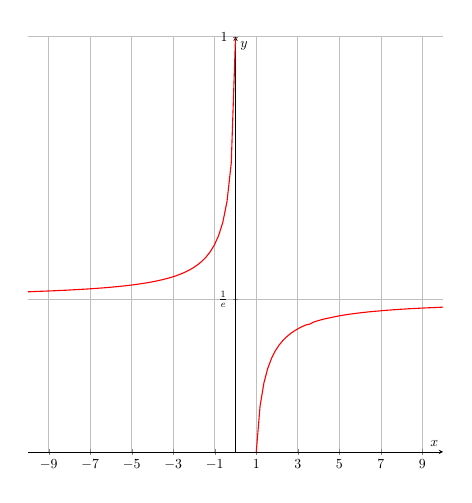
\begin{tikzpicture}[scale=.5]
		\begin{axis}[
			xmin=-10,xmax=10,
			ymin=0,ymax=1,
			grid=both,
			width=\textwidth,height=\textwidth,
			xlabel=$x$,
			ylabel=$y$,
			axis lines=middle,
			xtick={-9,-7,...,10},
			ytick={.3679,1},
			yticklabels={$\frac1e$,$1$},
		]
			\begin{scope}[samples=50,thick,red]
				\addplot[domain=-10:-0]{(1-1/x)^x};
				\addplot[domain=+1:+10]{(1-1/x)^x};
			\end{scope}
		\end{axis}
	\end{tikzpicture}
	\caption{函数\(y=\left(1-\tfrac1x\right)^x\)的图像}
\end{figure}
\begin{solution}
令\(t = -x\),
则当\(x \to +\infty\)时,
\(t \to -\infty\),
于是\[
	\lim_{x\to+\infty} \left(1-\frac1x\right)^x
	= \lim_{t\to-\infty} \left(1+\frac1t\right)^{-t}
	= \left[\lim_{t\to-\infty} \left(1+\frac1t\right)^t\right]^{-1}
	= \frac1e.
\]
\end{solution}
\end{example}

\begin{example}
计算极限\(\lim_{x\to0^-} \left(1-\frac1x\right)^x\).
\begin{solution}
直接计算得\[
	\lim_{x\to0^-} \left(1-\frac1x\right)^x
	\xlongequal{t=-1/x} \lim_{t\to+\infty} \frac{1}{\sqrt[t]{1+t}}
	= \left(\lim_{t\to+\infty} \sqrt[t]{1+t}\right)^{-1}
	= 1.
\]
\end{solution}
\end{example}

\begin{theorem}
%@see: 《数学分析(第7版 第一卷)》(卓里奇) P110 定理5(复合函数极限定理)
设\(\mathcal{B}_Y\)是集合\(Y\)中的基,
\(\mathcal{B}_X\)是集合\(X\)中的基,
映射\(g\colon Y\to\mathbb{R}\)在基\(\mathcal{B}_Y\)上有极限,
映射\(f\colon X\to Y\)满足
\((\forall B_Y\in\mathcal{B}_Y)
(\exists B_X\in\mathcal{B}_X)
[f(B_X) \subseteq B_Y]\),
则复合映射\(g \circ f\colon X\to\mathbb{R}\)在基\(\mathcal{B}_X\)上有极限,
且\[
	\lim_{\mathcal{B}_X} (g \circ f)(x)
	= \lim_{\mathcal{B}_X} g(f(x))
	= \lim_{\mathcal{B}_Y} g(y).
\]
\begin{proof}
设\(\lim_{\mathcal{B}_Y} g(y) = A\).
我们来证明\(\lim_{\mathcal{B}_X} g(f(x)) = A\).
按照点\(A\)的给定邻域\(V(A)\)求出基\(\mathcal{B}_Y\)的元素\(B_Y\),
使得\(g(B_Y) \subseteq V(A)\).
根据条件,可以求出基\(\mathcal{B}_X\)的元素\(B_X\),
使得\(f(B_X) \subseteq B_Y\).
但此时\((g \circ f)(B_X) = g(f(B_X)) \subseteq g(B_Y) \subseteq V(A)\),
这就说明\(A\)是\(g \circ f\)在基\(\mathcal{B}_X\)上的极限.
\end{proof}
\end{theorem}
